\renewcommand{\baselinestretch}{1.5}
\onehalfspacing
\fancypagestyle{plain}{
\fancyhf{}
\rhead{\thepage}
\renewcommand{\headrulewidth}{0pt}
\renewcommand{\footrulewidth}{0pt}
}

\chapter{Introduction}

\section{Background}

\subsection{Latent diffusion models}

A latent diffusion model (LDM) \cite{Rombach2022} separates image generation into two stages. First, an autoencoder is trained to compress an image $x \in \mathbb{R}^{H\times W\times C}$ into a compact latent $z = E(x)$ and to reconstruct it with a decoder $\hat{x} = D(z)$. Second, a generative model is trained in the latent space, so that new latents can be sampled and decoded into images. Working in the latent space reduces the cost of training and sampling with respect to diffusion in pixel space. In this work, a $256\times256$ crop is compressed into a latent of size $4\times32\times32$ (a $8\times$ spatial reduction with 4 channels), and each position of that grid is a \emph{token} in the terminology of the literature; the autoencoder is therefore also called a tokenizer.

\subsection{Variational autoencoders}

A variational autoencoder (VAE) \cite{Kingma2014} learns a probabilistic encoder $q_\phi(z\mid x)=\mathcal{N}(\mu_\phi(x),\sigma_\phi^2(x))$ and a decoder $p_\theta(x\mid z)$. It is trained by minimizing a reconstruction term plus a regularization term that keeps the latent close to a standard Gaussian prior:
\begin{equation}
\mathcal{L}_{\mathrm{VAE}} = \mathbb{E}_{q_\phi(z\mid x)}\big[\lVert x-\hat{x}\rVert_2^2\big] + \beta\, D_{\mathrm{KL}}\big(q_\phi(z\mid x)\,\Vert\,\mathcal{N}(0,I)\big),
\end{equation}
where the latent is sampled with the reparameterization $z=\mu_\phi(x)+\sigma_\phi(x)\odot\varepsilon$, $\varepsilon\sim\mathcal{N}(0,I)$. The weight $\beta$ controls the trade-off between reconstruction and regularization \cite{Higgins2017}; in this work $\beta=10^{-3}$. A discrete alternative replaces the Gaussian latent with a codebook of embeddings (VQ-VAE) \cite{vandenOord2017}.

\subsection{Adversarial training}

A generative adversarial network (GAN) \cite{Goodfellow2014} trains a discriminator $D_\psi$ to distinguish real from generated images while the generator is trained to fool it. When the discriminator judges local patches instead of the whole image \cite{Isola2017}, it encourages sharp local texture. In a VAE, an adversarial term can be added to the loss, $\mathcal{L}=\mathcal{L}_{\mathrm{VAE}}+\lambda\,\mathcal{L}_{\mathrm{adv}}$, with a small weight $\lambda$ (here $\lambda=0.01$).

\subsection{Diffusion and Flow Matching}

A denoising diffusion probabilistic model (DDPM) \cite{Ho2020} defines a forward process that gradually adds Gaussian noise to a latent $z_0$,
\begin{equation}
z_t=\sqrt{\bar{\alpha}_t}\,z_0+\sqrt{1-\bar{\alpha}_t}\,\varepsilon,\qquad \varepsilon\sim\mathcal{N}(0,I),
\end{equation}
and trains a network $\varepsilon_\theta$ to predict the added noise,
\begin{equation}
\mathcal{L}_{\mathrm{DDPM}}=\mathbb{E}_{z_0,\varepsilon,t}\big[\lVert\varepsilon-\varepsilon_\theta(z_t,t)\rVert_2^2\big].
\end{equation}
Sampling starts from pure noise and removes it step by step (here, with 1000 training steps). Flow Matching \cite{Lipman2023} instead learns a velocity field along a path between noise $x_0\sim\mathcal{N}(0,I)$ and data $x_1$. With the linear path $x_t=(1-t)\,x_0+t\,x_1$, the target velocity is constant, $v=x_1-x_0$, and the loss is
\begin{equation}
\mathcal{L}_{\mathrm{FM}}=\mathbb{E}_{x_0,x_1,t}\big[\lVert v_\theta(x_t,t)-(x_1-x_0)\rVert_2^2\big].
\end{equation}
Sampling integrates the learned velocity with a few Euler steps (here, 50), which makes generation considerably faster than DDPM sampling.

\subsection{Evaluation metrics}

The quality of the reconstruction is measured with the mean squared error (MSE) and the peak signal-to-noise ratio. The quality of the generated images is measured by comparing the distribution of generated images with that of real images in the feature space of an Inception network. The Fr\'echet Inception Distance (FID) \cite{Heusel2017} models both sets of features as Gaussians with means $\mu_r,\mu_g$ and covariances $\Sigma_r,\Sigma_g$:
\begin{equation}
\mathrm{FID}=\lVert\mu_r-\mu_g\rVert_2^2+\mathrm{Tr}\!\big(\Sigma_r+\Sigma_g-2(\Sigma_r\Sigma_g)^{1/2}\big).
\end{equation}
The Kernel Inception Distance (KID) \cite{Binkowski2018} is the squared maximum mean discrepancy with a polynomial kernel; unlike FID, it has an unbiased estimator and does not depend on the number of generated images in the same way, so it is more reliable for small samples. For both metrics, lower is better.

\section{Related Work}

% TODO (estado del arte): diseño del espacio latente; autoencoders con enmascarado y tratamientos de datos;
% generación con pocos datos y en agricultura; generación multimodal. Fuentes verificadas en docs/literature_map.md.

\subsection{Literature search}

\textbf{Review question.} Has the effect of data treatments and of structural modifications of the VAE on the generation quality of latent diffusion models been studied for small, homogeneous, and multimodal datasets?

\textbf{Source and date.} The arXiv API was queried on 11 October 2026, restricted to submissions from 2022 onward. All strings combine a latent-diffusion term (L) with a term for the autoencoder (A), plus the term specific to each string:
\begin{itemize}
  \item L = \texttt{all:"latent diffusion" OR abs:"latent diffusion model"}
  \item A = \texttt{abs:autoencoder OR abs:VAE OR abs:tokenizer}
\end{itemize}

\begin{table}[H]
\centering
\small
\begin{tabular}{p{0.06\textwidth}p{0.62\textwidth}p{0.18\textwidth}}
\hline
\textbf{ID} & \textbf{Search string (in addition to L)} & \textbf{Records} \\
\hline
S1 & A \texttt{AND (abs:augmentation OR abs:"data augmentation")} & 30 \\
S2 & A \texttt{AND (abs:adversarial OR abs:"KL" OR abs:regularization OR abs:"latent channels")} & 73 \\
S3 & A \texttt{AND (abs:aerial OR abs:agricultural OR abs:crop OR abs:plant OR abs:UAV OR abs:"remote sensing")} & 9 \\
S4 & \texttt{(abs:masked OR abs:masking) AND} A & 47 \\
S5 & \texttt{abs:depth AND (abs:RGB OR abs:appearance) AND (abs:joint OR abs:jointly OR abs:"shared latent")} & 7 \\
\hline
\end{tabular}
\caption{Search strings and number of records returned by arXiv. A first version of S1 and S2 that also required a small-data term was too restrictive (it returned an error and one record, respectively) and was replaced by the strings above.}
\end{table}

\textbf{Screening criteria.} Records were screened by title and abstract with three criteria:
\begin{enumerate}
  \item \textbf{C1:} the work varies something in the autoencoder or in its training data (augmentation, masking, adversarial loss, KL or regularization, number of latent channels, or fine-tuning).
  \item \textbf{C2:} the work measures generation (FID, KID, generation or sample quality, image generation or synthesis).
  \item \textbf{C3:} the work addresses few or homogeneous data (small or limited datasets, few images, scarcity, few-shot, data efficiency) or an aerial, agricultural, or medical domain.
\end{enumerate}
The screening was automatic: each criterion was a set of keywords applied to the title and abstract, and the abstracts of the records that met C1, C2, and C3 were then read by the author. A work is considered to study the review question when it meets the three criteria and examines how the data or the structure of the autoencoder change generation.

\textbf{Result.} Figure~\ref{fig:prisma} summarizes the flow. Of 151 unique records, 34 met C1 and C2, and 4 of them also met C3 or the domain; the four are medical applications that use a VAE to synthesize data and do not study the effect of its design or of the data treatments. No record studied the review question.

\begin{figure}[H]
\centering
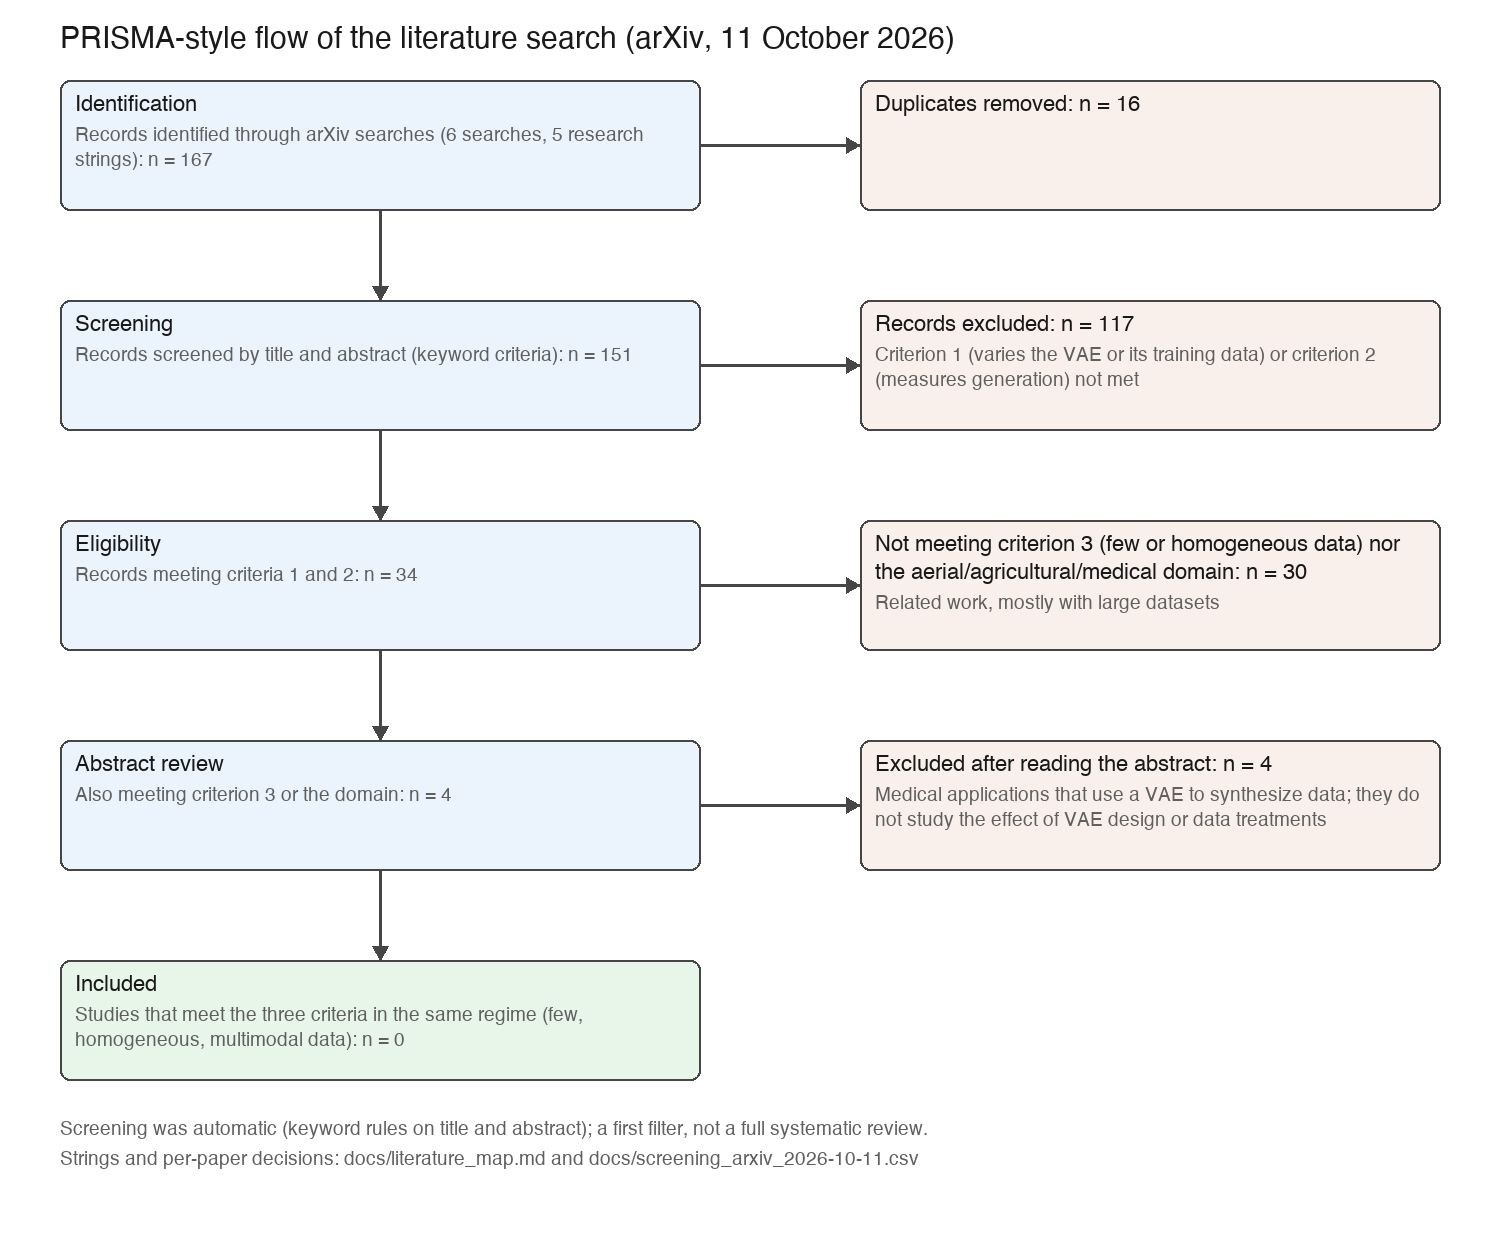
\includegraphics[width=0.95\textwidth]{Imagenes/prisma_arxiv.png}
\caption{PRISMA-style flow of the literature search on arXiv (11 October 2026). Screening was automatic, based on keyword rules over title and abstract.}
\label{fig:prisma}
\end{figure}

\textbf{Limitations.} Only arXiv was searched, the screening relied on keywords, and the search was not repeated by a second reviewer; it is a first systematic search and not a full systematic review.
